\section{A Changing Web}

Back when HTTP/1.1 was standardised in 1999, web pages generally consisted of a single file that included text and some directives to indicate how the page should be laid out when displayed by a browser, possibly accompanied by an image or two. Looking at the Wikipedia home page from 2001~\cite{wikiold}, we can see that this is true: a single image is displayed at the top right hand corner of the page, and everything else is simple text styling and some hyperlinks to other similar pages. A possible layout file (known as an HTML file) that could be used to display a single image is as follows:

\begin{minted}{html}
<img src="logo.png"/>
\end{minted}

This is the exact data\footnote{Most likely in the ASCII encoding, which means that each character of text is represented by one byte, which is equivalent to a number between 0 and 255 inclusive.} that the browser might receive from a server after requesting the homepage of a website. As you can see, the \mintinline{html}{<img>} tag simply references an image (specifying the source at a location called \texttt{logo.png}); it does not provide the actual image data. The browser must now request the image from the location specified in the \texttt{src} attribute before it can be displayed. So, after the HTML has been retrieved, the browser initiates another request for the image at the URL \texttt{https://some-website.com/logo.png}. When this second request finishes, the browser takes the image data and displays it to the user.

Websites have significantly increased in complexity over the last two decades. For example, a full page load of \url{https://amazon.com/} consists of 173 requests, transferring over 3.3 megabytes of data~\cite{requestchecker}. However, forcing the browser to initiate too many requests can quickly introduce large delays: on a single connection, only one request may be outstanding at any time, meaning that if a browser needs to request two images it must wait for the whole of the first response before it can initiate the second request, as opposed to sending off the two requests and receiving the two responses in parallel\footnote{This issue is known as `head of line blocking' and was already recognised as a problem when HTTP/1.1 was being standardised, but a method that was introduced to alleviate it was not implemented in any major browsers due to some misbehaving servers not handling these parallel requests properly~\cite{pipelining}.}. In the former case, the total page load time is directly proportional to the number of requests made, whereas in the latter case the total page load time is independent of the number of requests and therefore scales much better on websites like Amazon that force the browser to start hundreds of requests upon every page load.

Due to this inability to process parallel requests on a single connection, browsers began doing the next logical thing: opening more connections. HTTP/1.1 specified a limit of 2 connections at a time~\cite[\S~8.1.4]{h1}, but today most browsers ignore this limit, using a maximum of 4 to 8 connections depending on the browser~\cite{maxconnections}.

This is the first of the major differences between HTTP/1.1 and HTTP/2. In the former, parallelism is achieved through opening multiple connections to the server. In the latter, all operations are instead conducted over a single connection in such a way that requests and responses can be interleaved in whichever way is most convenient to the client or server~\cite[\S~1]{h2}. In cases where the browser is performing more requests than the maximum number of connections it is permitted to open, using HTTP/2 can yield very high performance gains.

Another reason why using one connection is preferable to using multiple connections is due to the time it takes to open a connection. If the client and server want to communicate using encryption, the client and server must perform a `handshake' to negotiate the ciphers and cryptographic keys that will be used, which has been shown to increase the median time it takes to open a connection by roughly 3 times the round trip time\footnote{Also known as RTT, latency or ping: this is a measure of how long it takes for a single byte of data to be sent from a client to a server and back.}~\cite{tlsoverhead}, potentially adding a 50 to 500 milliseconds delay depending on the distance between the server and the client.

As a practical demonstration of the performance gains that are to be made, I have set up a web page (using the web server I have created) at \url{https://mattst.me/tiles.html} which consists of a large image split into 180 smaller images. This forces the browser to very quickly max out the number of parallel requests that it can use, which gives HTTP/2 a significant advantage since by default there is no limit to the number of parallel requests that can be active at a time. You can click on the buttons to switch between using HTTP/1.1 and HTTP/2, and observe the time taken at the bottom of the page. On my computer, the `time taken' to fully load the page varies with round trip time as follows (all results averaged over 5 readings):

\begin{table}[h!]
\begin{center}
\begin{tabular}{|c|c|c|}
	\hline
	Round trip time/ms & HTTP/1.1 time taken/s & HTTP/2 time taken/s \\
	\hline
	14 & 0.914 & 0.399 \\
	\hline
	30 & 1.449 & 0.535 \\
	\hline
	60 & 2.430 & 0.694 \\
	\hline
	100 & 3.746 & 0.930 \\
	\hline
	200 & 6.909 & 1.515 \\
	\hline
	500 & 16.508 & 3.176 \\
	\hline
	1000 & 32.577 & 6.205 \\
	\hline
\end{tabular}
\caption{Mean page load time versus latency for HTTP/1.1 and HTTP/2 \\ \textit{(Arch Linux x86\_64, Chrome 64-bit 63.0.3239.108)}}
\end{center}
\end{table}

\begin{figure}
	\centering
	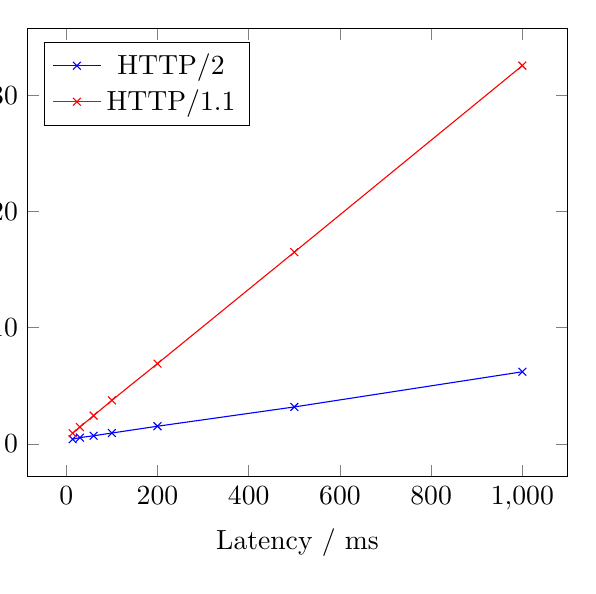
\begin{tikzpicture}[trim axis left, trim axis right]
		\begin{axis}[xlabel={Latency / ms}, ylabel={Mean page load time / s}, legend pos=north west]
			\addplot+ [mark=x, color=blue]
				coordinates {
					(14, 0.399)
					(30, 0.535)
					(60, 0.694)
					(100, 0.930)
					(200, 1.515)
					(500, 3.176)
					(1000, 6.205)
				};

			\addplot+ [mark=x, color=red]
				coordinates {
					(14, 0.914)
					(30, 1.449)
					(60, 2.430)
					(100, 3.746)
					(200, 6.909)
					(500, 16.508)
					(1000, 32.577)
				};

			\legend{HTTP/2,HTTP/1.1}
		\end{axis}
	\end{tikzpicture}
	\caption{Mean page load time versus latency for HTTP/1.1 and HTTP/2 \\ \textit{(Arch Linux x86\_64, Chrome 64-bit 63.0.3239.108)}}
\end{figure}

Here one can see that the head of line blocking effect in HTTP/1.1 becomes significantly more pronounced when high latencies are involved, since the client has to wait for full responses before sending off the next batch of requests. This feature is undoubtedly a great benefit to companies, especially given that there are now more people on mobile phones accessing the internet than there are people on desktop PCs accessing the internet~\cite{mobilephones}, and the WiFi or 3G/4G connections that phones use often incur higher latencies and have a higher chance of data needing to be re\hyp{}transmitted due to (among other things) poor reception~\cite{ethvswifi}.

Additionally, it may be interesting to consider the effects that this will have on the loading of advertisement. The Internet Advertising Bureau found that in February 2017, 22.1\% of UK adults were using ad blocker software~\cite{adblockuk}, which is software that blocks HTTP requests to servers that are known to distribute advertising. One reason for this is that blocking these unnecessary requests decreases page load time significantly~\cite{brave}, but with HTTP/2 this effect is reduced. Since ad blocking is forecast to cause revenue losses to UK publishers of \pounds 1.3 billion by 2020~\cite{adblockrevenue}, decreasing the appeal of ad blocking software is in their interest. 
